% Options for packages loaded elsewhere
\PassOptionsToPackage{unicode}{hyperref}
\PassOptionsToPackage{hyphens}{url}
%
\documentclass[
  12pt,
]{article}
\usepackage{lmodern}
\usepackage{amssymb,amsmath}
\usepackage{ifxetex,ifluatex}
\ifnum 0\ifxetex 1\fi\ifluatex 1\fi=0 % if pdftex
  \usepackage[T1]{fontenc}
  \usepackage[utf8]{inputenc}
  \usepackage{textcomp} % provide euro and other symbols
\else % if luatex or xetex
  \usepackage{unicode-math}
  \defaultfontfeatures{Scale=MatchLowercase}
  \defaultfontfeatures[\rmfamily]{Ligatures=TeX,Scale=1}
\fi
% Use upquote if available, for straight quotes in verbatim environments
\IfFileExists{upquote.sty}{\usepackage{upquote}}{}
\IfFileExists{microtype.sty}{% use microtype if available
  \usepackage[]{microtype}
  \UseMicrotypeSet[protrusion]{basicmath} % disable protrusion for tt fonts
}{}
\makeatletter
\@ifundefined{KOMAClassName}{% if non-KOMA class
  \IfFileExists{parskip.sty}{%
    \usepackage{parskip}
  }{% else
    \setlength{\parindent}{0pt}
    \setlength{\parskip}{6pt plus 2pt minus 1pt}}
}{% if KOMA class
  \KOMAoptions{parskip=half}}
\makeatother
\usepackage{xcolor}
\IfFileExists{xurl.sty}{\usepackage{xurl}}{} % add URL line breaks if available
\IfFileExists{bookmark.sty}{\usepackage{bookmark}}{\usepackage{hyperref}}
\hypersetup{
  pdftitle={Neighborhoods and Felony Disenfranchisement: The Case of New York City},
  pdfauthor={Kevin Morris},
  hidelinks,
  pdfcreator={LaTeX via pandoc}}
\urlstyle{same} % disable monospaced font for URLs
\usepackage[margin=1in]{geometry}
\usepackage{longtable,booktabs}
% Correct order of tables after \paragraph or \subparagraph
\usepackage{etoolbox}
\makeatletter
\patchcmd\longtable{\par}{\if@noskipsec\mbox{}\fi\par}{}{}
\makeatother
% Allow footnotes in longtable head/foot
\IfFileExists{footnotehyper.sty}{\usepackage{footnotehyper}}{\usepackage{footnote}}
\makesavenoteenv{longtable}
\usepackage{graphicx}
\makeatletter
\def\maxwidth{\ifdim\Gin@nat@width>\linewidth\linewidth\else\Gin@nat@width\fi}
\def\maxheight{\ifdim\Gin@nat@height>\textheight\textheight\else\Gin@nat@height\fi}
\makeatother
% Scale images if necessary, so that they will not overflow the page
% margins by default, and it is still possible to overwrite the defaults
% using explicit options in \includegraphics[width, height, ...]{}
\setkeys{Gin}{width=\maxwidth,height=\maxheight,keepaspectratio}
% Set default figure placement to htbp
\makeatletter
\def\fps@figure{htbp}
\makeatother
\setlength{\emergencystretch}{3em} % prevent overfull lines
\providecommand{\tightlist}{%
  \setlength{\itemsep}{0pt}\setlength{\parskip}{0pt}}
\setcounter{secnumdepth}{5}
\usepackage{rotating}
\newcommand{\beginsupplement}{\setcounter{table}{0}  \renewcommand{\thetable}{A\arabic{table}} \setcounter{figure}{0} \renewcommand{\thefigure}{A\arabic{figure}}}
\usepackage{setspace}\doublespacing
\usepackage{booktabs}
\usepackage{longtable}
\usepackage{array}
\usepackage{multirow}
\usepackage{wrapfig}
\usepackage{float}
\usepackage{colortbl}
\usepackage{pdflscape}
\usepackage{tabu}
\usepackage{threeparttable}
\usepackage{threeparttablex}
\usepackage[normalem]{ulem}
\usepackage{makecell}
\usepackage{xcolor}
\newlength{\cslhangindent}
\setlength{\cslhangindent}{1.5em}
\newenvironment{cslreferences}%
  {\setlength{\parindent}{0pt}%
  \everypar{\setlength{\hangindent}{\cslhangindent}}\ignorespaces}%
  {\par}

\title{Neighborhoods and Felony Disenfranchisement: The Case of New York City}
\author{Kevin Morris\footnote{The author thanks Jacob Faber, Jeff Manza, Myrna Pérez, Ariel White, and Peter Miller for their comments on this project. All errors are my responsibility.}}
\date{March 03, 2020}

\begin{document}
\maketitle
\begin{abstract}
Over the past two decades, scholars have sought to estimate the direct and indirect effects of felony disenfranchisement on political representation. This literature, however, has often overlooked both the geographic concentration of communities impacted by over-incarceration and the low propensity to vote exhibited by individuals convicted of felony crimes. In this paper, I redefine ``lost voters'' as disenfranchised individuals with a history of participating in elections. I map these individuals to their pre-incarceration addresses and use matching and linear models to explore whether their home neighborhoods turned out at lower rates than other neighborhoods. I find that neighborhoods that were home to lost voters turnout at substantially lower rates than similar neighborhoods, and that black neighborhoods are particularly impacted by the spillover effects of disenfranchisement. These indirect effects of the incarceration of would-be voters may have serious implications for the representation of impacted neighborhoods.
\end{abstract}

\pagenumbering{gobble}
\pagebreak

\pagenumbering{arabic}

\hypertarget{introduction}{%
\section*{Introduction}\label{introduction}}
\addcontentsline{toc}{section}{Introduction}

The political history of the United States has been characterized by a general, if nonlinear, trend toward universal suffrage (see, for instance, Keyssar \protect\hyperlink{ref-Keyssar2009}{2009}). At the time of the nation's founding, access to the ballot box was restricted to landed White men; over the following two centuries, the franchise was greatly expanded. Today, voting rights are considered foundational aspects of full citizenship (United Nations General Assembly Resolution 2200 (XXI)). Despite the United State's march toward ever-more-inclusive systems of democracy, however, one large group of American citizens is formally barred from voting. In most of the United States, citizens convicted of felonies are at least temporarily prohibited from casting ballots in elections (Brennan Center for Justice \protect\hyperlink{ref-bcj_laws}{2019}). Although some states such as Florida and Louisiana have gradually moved to dismantle their systems of felony disenfranchisement, an estimated 4.7 million American citizens remain disenfranchised (Uggen, Larson, and Shannon \protect\hyperlink{ref-sentencing_2016}{2016}).

Due to economic and racial segregation, these effects are highly spatially concentrated. Data available from New York City shows that in 2017, 10 of the New York Police Department's 77 precincts were responsible for more than a quarter of all arrests for felony charges. Many scholars have detailed the impact of living in areas with high levels of police activity. Residents of such neighborhoods suffer from worse physical health (Sewell and Jefferson \protect\hyperlink{ref-Sewell2016}{2016}) and are more likely to suffer from anxiety and exhibit symptoms of trauma (Geller et al. \protect\hyperlink{ref-Geller2014}{2014}). The labor markets and social networks in neighborhoods with high levels of policing and incarceration are disrupted (Clear \protect\hyperlink{ref-Clear2008}{2008}), while concentrated policing has also been credited with having a ``chilling effect'' on neighborhoods' willingness to reach out for help to local governments (Lerman and Weaver \protect\hyperlink{ref-Lerman2013}{2013}). Perhaps most troubling of all, these effects are not concentrated in random neighborhoods; as Gelman, Fagan, and Kiss (\protect\hyperlink{ref-Gelman2007}{2007}) shows, for instance, New York's ``stop-and-frisk'' policy impacted Black and Latino New Yorkers at rates far higher than Whites, even after controlling for neighborhood variability and race-specific arrest rates. The result is an incarcerated population that looks far different than the rest of the state: according to data from the New York State Department of Corrections and Community Supervision, 49.5 percent of individuals who were incarcerated in December of 2018 were non-Hispanic Black, although the Census Bureau estimates that just 14.3 percent of the citizen voting age population in the state is non-Hispanic Black.\footnote{Latinos are also over-represented among the incarcerated population, though not as dramatically: Latinos make up 14.1 percent of the citizen voting age population and 22.9 percent of the incarcerated population.}

Felony disenfranchisement policies are part of a criminal justice system that disproportionately impacts Black Americans living in certain communities. The effects of disenfranchisement are concentrated in neighborhoods that already suffer from myriad disadvantages thanks to social and economic marginalization. The neighborhood-specific implications of felony disenfranchisement, however, remain largely unstudied. A number of studies have explored the effect of imprisonment and disenfranchisement on later political participation (White \protect\hyperlink{ref-White2019}{2019}\protect\hyperlink{ref-White2019}{b}; Gerber et al. \protect\hyperlink{ref-Gerber2015}{2015}; Burch \protect\hyperlink{ref-Burch2011}{2011}). Others have looked at the spillover effects of disenfranchisement on eligible Black voters at the state level (Bowers and Preuhs \protect\hyperlink{ref-Bowers2009}{2009}; King and Erickson \protect\hyperlink{ref-King2016}{2016}). With the exception of Burch (\protect\hyperlink{ref-Burch2013}{2013}), however, little attention has been paid to the impact of felony disenfranchisement on political participation at the neighborhood level.

\hypertarget{background}{%
\section*{Background}\label{background}}
\addcontentsline{toc}{section}{Background}

Since the 2000 election, scholars have attempted to quantify the effect of felony disenfranchisement on the political representation of highly-incarcerated communities. Uggen and Manza (\protect\hyperlink{ref-Uggen2002}{2002}) produced the first estimates of felony disenfranchisement's impact on turnout, arguing that Al Gore would have won the presidency if not for disenfranchisement in Florida. Their analysis estimated the direct effects of felony disenfranchisement on turnout by quantifying the number of actually disenfranchised individuals who would have participated if given the chance. Since Uggen and Manza (\protect\hyperlink{ref-Uggen2002}{2002}), other scholars have also investigated the direct effect of felony disenfranchisement (Miles \protect\hyperlink{ref-Miles2004}{2004}; Uggen and Manza \protect\hyperlink{ref-Uggen2004}{2004}; Drucker and Barreras \protect\hyperlink{ref-Drucker2005}{2005}; Ochs \protect\hyperlink{ref-Ochs2006}{2006}).

This paper begins by exploring the effect of felony disenfranchisement on neighborhood turnout in the New York City Mayoral election of 2017 using individual-level administrative data. Policing and incarceration patterns have historically targeted communities of color, damaging the social fabric of these neighborhoods (e.g.~Sewell and Jefferson \protect\hyperlink{ref-Sewell2016}{2016}; Clear \protect\hyperlink{ref-Clear2008}{2008}; Lerman and Weaver \protect\hyperlink{ref-Lerman2013}{2013}). It is possible, however, that these effects run deeper than the direct focus on policing and incarceration has acknowledged. We know that felony disenfranchisement systematically removes individuals from certain neighborhoods, but it is not clear that enough would-be voters are removed relative to the electorate to meaningfully distort neighborhood representation. To the extent that felony disenfranchisement has a spatially-concentrated depressive effect on eligible voters, it is possible that these policies are powerful enough to materially reduce the representation of certain parts of the city.

\hypertarget{framing-for-turnout-effects}{%
\section*{Framing for Turnout Effects}\label{framing-for-turnout-effects}}
\addcontentsline{toc}{section}{Framing for Turnout Effects}

Despite over-incarceration in some neighborhoods, the number of incarcerated individuals is relatively low compared to the number of voters. In New York, for instance, 46,232 individuals were imprisoned in New York State in early 2019, compared with 11.6 million actively registered voters. Despite the low share of residents who are directly disenfranchised, there is reason to believe the policy impacts more individuals than just those imprisoned. As discussed above, previous research has demonstrated that felony disenfranchisement reduces turnout even among Black voters whose rights are not suspended This research has found, in particular, that eligible Black voters are less likely to cast a ballot in states where felony disenfranchisement policies are harsher, an effect often referred to as \emph{de facto} disenfranchisement.

Though previous studies have focused largely on the state-level spill-over effects of felony disenfranchisement, there is reason to believe that this \emph{de facto} disenfranchisement is concentrated within the neighborhoods home to formally disenfranchised residents. Burch (\protect\hyperlink{ref-Burch2013}{2013}), for instance, demonstrates that neighborhoods in North Carolina with higher levels of incarceration had lower turnout. Moreover, voting is a social act, and social networks play an important role in predicting political participation (e.g.~Foladare \protect\hyperlink{ref-Foladare1968}{1968}; Huckfeldt \protect\hyperlink{ref-Huckfeldt1979}{1979}; Kenny \protect\hyperlink{ref-Kenny1992}{1992}; Mutz \protect\hyperlink{ref-Mutz2002}{2002}). Literature from urban sociology has established that social networks are largely spatially bounded, and that local social ties are more important in lower-income neighborhoods (Guest and Wierzbicki \protect\hyperlink{ref-Guest1999}{1999}; Dawkins \protect\hyperlink{ref-Dawkins2006}{2006}). It should be no surprise, then, that neighborhoods have been shown to mobilize and demobilize voters through mechanisms above-and-beyond individual characteristics (Gimpel, Dyck, and Shaw \protect\hyperlink{ref-Gimpel2004}{2004}; Cho, Gimpel, and Dyck \protect\hyperlink{ref-Cho2006}{2006}). To the extent that felony disenfranchisement policies have depressive effects on turnout in the social and filial networks of the imprisoned and paroled, these effects are likely to be closely concentrated in the neighborhoods where the disenfranchised live. I therefore hypothesize that felony disenfranchisement does have locally bounded spillover effects, and that turnout in neighborhoods with lost voters systematically vote at a lower rate than others.

Recent work from Hannah Walker and others, however, leads me to moderate my hypothesis about the indirect neighborhood effects of lost voters. Walker (\protect\hyperlink{ref-Walker2014}{2014}) and Walker and García-Castañon (\protect\hyperlink{ref-Walker2017}{2017}), for instance, demonstrate that individuals who have proximal contact with the criminal justice system (defined as ``as having a loved one who is a custodial citizen without yourself having had contact'' (Walker and García-Castañon \protect\hyperlink{ref-Walker2017}{2017}, 542)) were not less likely to vote, but \emph{were} more likely to participate in nonelectoral political events (such as signing a petition, attending a community meeting, or writing to an elected official). These effects are particularly pronounced for women of color. Although Walker and others demonstrate that these actions largely take place outside of the voting booth, they may moderate spillover effects on turnout.

Similarly, White (\protect\hyperlink{ref-White2019a}{2019}\protect\hyperlink{ref-White2019a}{a}) finds that incarceration has only moderate indirect effects on voting. She finds ``evidence of a short-term demobilization effect for people who see household members convicted or jailed in the weeks before the election, but no evidence of a lasting turnout effect from these experiences'' (607). This study does not, however, interrogate whether the incarceration of a would-be voter has different indirect effects than the incarceration of an individual who would not have voted either way. It is possible that the indirect effects of the incarceration or jailing of a would-be voter are different than the indirect effects arising from other individuals. Nevertheless, the literature on the effects of proximal contact with the criminal justice system and felony disenfranchisement is hardly settled.

\hypertarget{methodology-and-data}{%
\section*{Methodology and Data}\label{methodology-and-data}}
\addcontentsline{toc}{section}{Methodology and Data}

To identify lost voters, and to determine whether lost voters reduce neighborhood turnout, I use data provided directly by the State of New York.

The first dataset is from the Department of Corrections and Community Supervision (DOCCS). This data includes information on every individual who was incarcerated in state prison, or on parole after serving time in state prison. These data include individuals' first, middle, and last names, as well as their date of birth, the dates they spent incarcerated or on parole, and other information. I limit the records in the data to include all individuals who were either in prison or on parole as of the mayoral election in 2017.

The second primary dataset is the registered voter file from New York State. The registered voter file includes information on every voter registered in the state such as name, address, vote history, and gender. It also includes the records of everyone who has been purged --- in other words, whose registration has been cancelled. The records are marked as ``purged,'' and allow me to identify the vote history even of individuals who have been purged for a felony conviction.

By matching these two datasets using first, middle, and last names, and date of birth, I can identify all individuals who were disenfranchised in the City of New York on election day in 2017 \emph{who had a history of voting.} Specifically, a ``lost voter'' is someone who cast a ballot between January 1, 2007 and December 31, 2016 and was imprisoned or on parole for a felony offense on November 7\textsuperscript{th}, 2017.

\hypertarget{why-do-we-care-about-lost-voters}{%
\section*{Why Do We Care About ``Lost Voters''?}\label{why-do-we-care-about-lost-voters}}
\addcontentsline{toc}{section}{Why Do We Care About ``Lost Voters''?}

In this analysis, I offer a different definition of ``lost voter'' than much of the literature. Many recent papers have attempted to identify relationships between the number of disenfranchised residents --- \emph{potentially} lost voters --- and turnout. Such an approach is informative for understanding the impact of disenfranchisement. Many young men, for instance, are admitted to prison each year. If someone is incarcerated shortly after they turn 18 in an odd-numbered year, they may be incarcerated before they even have the opportunity to cast a ballot. Similarly, we know that older individuals are more likely to vote; if someone who is incarcerated would have ``aged in'' to voting but for their incarceration, they will have no history of voting. This analytical approach is also often taken due to data constraints: most states' registered voter files provide only a snapshot of currently registered voters, making it impossible to determine voting history for individuals who are currently disenfranchised (and therefore not currently registered). Similarly, state-level data does not report the number of incarcerated individuals with a history of voting; therefore, studies that leverage variation in laws between states to estimate the effect of felony disenfranchisement rely on estimates of the total disenfranchised population, not the number of disenfranchised individuals with a history of voting.

Examining the impact of all disenfranchised voters, however, limits our ability to understand the specific direct and indirect causal effects of felony disenfranchisement. As previous research has detailed, turnout rates among individuals who are incarcerated are very low even prior to incarceration (e.g.~Gerber et al. \protect\hyperlink{ref-Gerber2017}{2017}). Research showing lower turnout where more individuals are formally disenfranchised might only be identifying the indirect effects of incarceration on turnout. Estimation of the effects of felony disenfranchisement above-and-beyond the effects of incarceration must account for the low propensity to vote among the formally disenfranchised.

Here, I explore whether the disenfranchisement of residents with a history of participating in elections is related to neighborhood turnout. In this analysis, ``lost voters'' are individuals ineligible to cast a ballot on a given election day who have cast a ballot in the previous ten years. Although not all lost voters would have participated if they had not been disenfranchised, past participation is an extremely strong predictor of propensity to vote (Gerber, Green, and Shachar \protect\hyperlink{ref-Gerber2003}{2003}). As such, these are the individuals most likely to have been directly impacted not only by incarceration but specifically by felony disenfranchisement. Identifying the effects of felony disenfranchisement in neighborhoods that lost individuals with a record of voting --- individuals who would likely have cast a ballot had they been allowed --- provides insight into whether felony disenfranchisement reduces neighborhood turnout. Because New York State's voter file includes information on individuals who have been purged for felony convictions, I can reconstruct the vote history even for voters who are no longer eligible to vote.

Of course, the incarceration of neighbors and family members who have \emph{not} voted in the past might also have indirect effects on neighborhood turnout rates. Even if an eligible New Yorker's incarcerated brother would not have voted, for instance, the eligible voter might not cast a ballot due to a soured impression of the political process. Such an indirect effect, however, would arise from the incarceration and not from the disenfranchisement of a voter. Here, I am isolating the direct effect of felony disenfranchisement.

\hypertarget{geocoding}{%
\section{Geocoding}\label{geocoding}}

After the lost voters have been identified, the full registered voter file is geocoded by SmartyStreets, which successfully geocoded 99 percent of all voters. Figure \ref{fig:citywide-map} shows the geographical distribution of the lost voters.

\begin{figure}[H]

{\centering 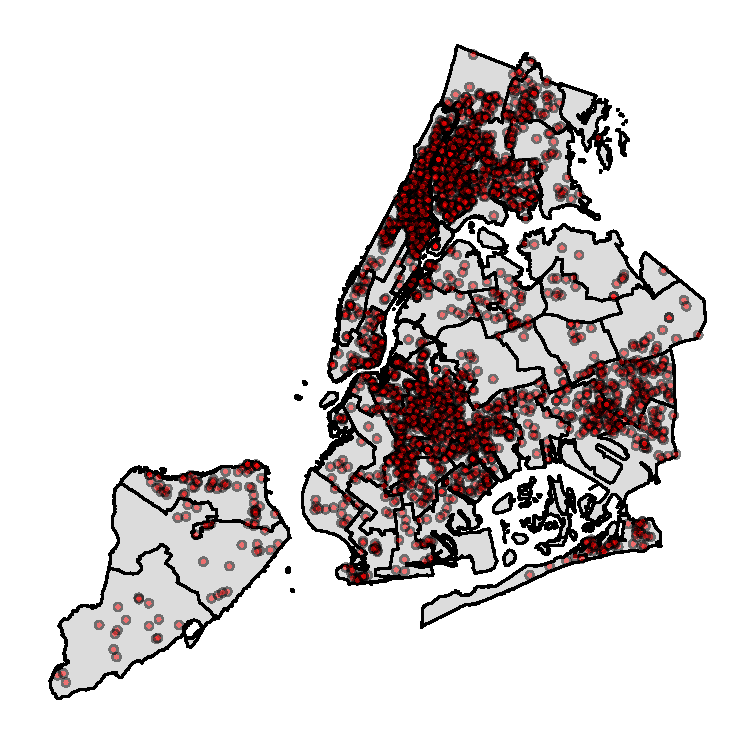
\includegraphics{for_brennan_files/figure-latex/citywide-map-1} 

}

\caption{\label{fig:citymap}Lost Voters on Election Day, 2017}\label{fig:citywide-map}
\end{figure}

Although 73,223 individuals were formally disenfranchised as of the 2017 election, there were just 6,166 disenfranchised voters statewide who had participated in the past 10 years.\footnote{Because address prior to incarceration is not available for individuals who were not registered to vote, computing the total number of formally disenfranchised individuals in New York City is not possible.} Just 8.4 percent of formally disenfranchised individuals, therefore, were individuals with a demonstrated history of participating.

The spatial concentration of lost voters is readily apparent. In some communities, such as Greenwich Village and Brooklyn Heights, hardly any voters were disqualified from participating in the 2017 elections. In other communities, such as Harlem and Central Brooklyn, large numbers of individuals with a demonstrated history of voting were not allowed to cast a ballot for mayor.

\hypertarget{results}{%
\section*{Results}\label{results}}
\addcontentsline{toc}{section}{Results}

After determining lost voters' geographic coordinates, I determine the Census block group in which they live. I then aggregate these numbers up to determine the total number of lost voters residing in each block group in New York City. In Table \ref{tab:trad-reg} below, I adopt a standard ordinary least squares regression to investigate whether lost voters are associated with lower turnout rates in the 2017 election. In addition to the number of lost voters a neighborhood has, I include other sociodemographic characteristics from the Census Bureau's American Community Survey for the 5 years ending in 2017. Neighborhood-level turnout is calculated by aggregating the number of votes cast according to the geocoded voter file, and dividing that number by the citizen voting age population. Robust standard errors are clustered by city council district.\footnote{Where neighborhoods cross city council district lines, they are assigned the district in which most of their voters live for clustering purposes.}

Model 1 includes an un-interacted estimate of the number of lost voters as the primary dependent variable. Model 2, however, asks whether the effect of lost voters operates differently in Black communities. Prior research indicates that this might be the case, so the primary independent variable --- the number of lost voters --- is interacted in Model 2 with the share of the neighborhood that is non-Hispanic Black.

\begin{singlespace}

\input{"../../temp/table2.tex"}
\end{singlespace}

As Table \ref{tab:trad-reg} shows, lost voters are generally associated with lower turnout. Each missing voter in a block group reduces that neighborhood's turnout by about 0.82 percentage points. Model 2, however, makes clear that this effect is concentrated in Black neighborhoods. In neighborhoods where most residents are Black, each lost voter is associated with a turnout decrease of up to 1.87 percentage points. The neighborhoods most affected by felony disenfranchisement are neighborhoods where incarceration patterns overlap with Black communities.

The block groups where these depressive effects are concentrated are not randomly distributed throughout the city. They are highly spatially concentrated in Central Brooklyn, Eastern Queens, and Harlem. Figure \ref{fig:postest} applies the coefficient on \(Lost\ Voters \times Share\ Black\) from Model 2 in Table \ref{tab:trad-reg} to the city's block groups. The estimated depressive effect is \(-0.019\times Lost\ Voters \times Share\ Black\).

\begin{figure}[H]

{\centering 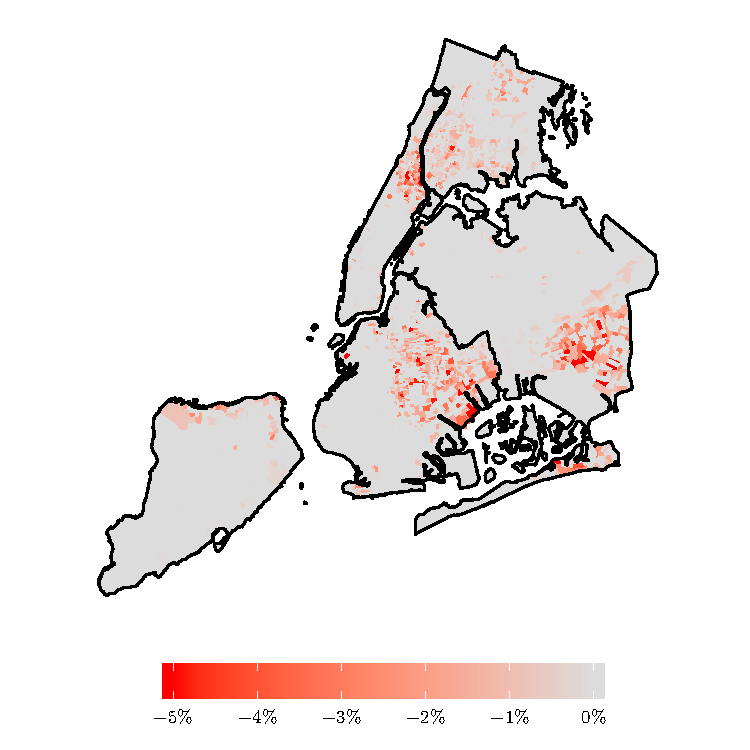
\includegraphics{for_brennan_files/figure-latex/postest-map-1} 

}

\caption{\label{fig:postest}Estimated Depressive Effect of Felony Disenfranchisement}\label{fig:postest-map}
\end{figure}

\hypertarget{discussion}{%
\section*{Discussion}\label{discussion}}
\addcontentsline{toc}{section}{Discussion}

During the 2017 mayoral election, felony disenfranchisement laws were responsible for removing an estimated 2,518 voters from New York City neighborhoods. The spatial concentration of these lost voters is striking, as demonstrated in Figure \ref{fig:citywide-map}, and the systematic removal of voters from these neighborhoods is troubling. However, more than one million votes were cast in the general election of 2017. Although felony disenfranchisement rules have implications for the individuals targeted by them, the removal of such a small number of voters --- concentrated though they are --- is unlikely to have large implications on its own.

As this analysis makes clear, however, felony disenfranchisement reaches beyond the individuals who are incarcerated. Previous literature has established that felony disenfranchisement impacts Black turnout at the state level, but this analysis demonstrates that these demobilizing effects intersect with geographical space to systematically depress the vote in neighborhoods where voters are being sent to prison. As discussed above, these neighborhoods have far lower incomes than the rest of the city: the median income of block groups without any lost voters is more than 40 percent higher than the median income of block groups with lost voters. Similarly, just 17 percent of individuals in the average block group with a lost voter were White, compared with 40 percent of the population in other block groups. Felony disenfranchisement has spillover effects on neighborhood turnout, and these neighborhoods systematically differ from the rest of the city's population. The effects are concentrated in neighborhoods where the most marginalized members of society live. These highly concentrated spillover effects are cause for major concern.

Of equal concern is the apparent concentration of these effects in Black neighborhoods. Table \ref{tab:trad-reg} indicates that once the lost voter indicator is interacted with the share of a neighborhood that is non-Hispanic Black, the lost voter indicator is either nonsignificant or significant and positive. This means that lost voters have no spillover effects in neighborhoods with small Black populations. Understanding the magnitude of this finding is important. In New York City, there are 1386 block groups where the Black community makes up more than 38 percent of the population (the average for treated block groups), with an average of 912 voting age citizens. In an average block group that is 38 percent Black, each lost voter cost the neighborhood 6.5 ballots. In block groups of the same size where the population is just 16 percent Black, lost voters cost the neighborhood just 1.6 ballots --- hardly more votes than the lost voter herself.

Why do lost voters in Black neighborhoods have such large spillover effects, when lost voters in predominantly non-Black neighborhoods do not? Much of the previous literature in this space establishes that individuals who have negative interactions with the government are less likely to choose to interact with the state in the future --- that these interactions have large ``interpretive effects'' (Pierson \protect\hyperlink{ref-Pierson1993}{1993}). Lerman and Weaver (\protect\hyperlink{ref-Lerman2013}{2013}), for instance, shows that neighborhoods where there are many police stops that involve searches or use of force use 311 services less frequently. Weaver and Lerman (\protect\hyperlink{ref-Weaver2010}{2010}) argues that interactions with the criminal justice system changes how individuals understand both their identities as citizens and the nature of governmental structures. Similarly, Lerman and Weaver (\protect\hyperlink{ref-Lerman2014}{2014}) tells us that those who have had contact with the criminal justice system consider political participation not just unfruitful but rather ``as something to be actively avoided'' (16). It is perhaps unsurprising that the negative spillover effects are largest in neighborhoods where police presence and criminal justice involvement is most keenly (and unfairly) felt; namely, in plurality and majority Black neighborhoods.

Individuals who live in neighborhoods where police activity is relatively limited may interpret the incarceration of a neighbor as a largely individual phenomenon. If it is understood as an isolated or individual event, voters in these neighborhoods who are not incarcerated are not likely to update their view of the state. They may draw no connections between their neighbor's imprisonment and their own efficacy as a voter. In the neighborhoods where policing is most prevalent --- often, lower-income Black communities --- the incarceration of a neighbor might not be interpreted so individualistically. It may, rather, be interpreted as another reminder of the government's unfairness. If a would-be voter finds herself soured on political participation because of her neighbor's incarceration, she may be less likely to cast a ballot.

This finding mirrors White (\protect\hyperlink{ref-White2019}{2019}\protect\hyperlink{ref-White2019}{b}), which finds that brief jail spells decrease future participation more for Black individuals than for White individuals. This is perhaps unsurprising. A large body of research indicates that, even after controlling for various sociodemographic characteristics and interactions with the police, Black Americans have far more negative views of the criminal justice system than White Americans (e.g.~Browning and Cao \protect\hyperlink{ref-Browning1992}{1992}; Hurwitz and Peffley \protect\hyperlink{ref-Hurwitz2005}{2005}; Henderson et al. \protect\hyperlink{ref-Henderson1997}{1997}; Wu, Sun, and Triplett \protect\hyperlink{ref-Wu2009}{2009}). Experience with the criminal justice system is less likely to be viewed in isolation (and therefore more likely to affect voting patterns) in Black neighborhoods. There is therefore strong reason to suspect that the concentrated depressive effects of felony disenfranchisement in Black neighborhoods arise from these distinct interpretations of the act of incarceration by the state.

For decades, scholars have detailed the problems associated with poor and segregated urban neighborhoods (Wilson \protect\hyperlink{ref-Wilson1990}{1990}). More recent work has begun to interrogate the ways in which the increasing reach of the carceral state shapes the economic and political behavior of individuals caught up in the criminal justice system and their community members. Much of this work, however, has focused on either the impacts of living in marginalized communities (by measuring health and economic impacts) or has not accounted for the importance of physical space (by focusing only on proximal social, and not geographic, contact with directly impacted individuals). This analysis allows us to understand the implications for living in a neighborhood where individuals likely to cast a ballot are not allowed to because of a felony conviction. I find that neighborhoods that are home to lost voters --- and particularly neighborhoods with large Black populations --- systematically turn out for local elections at lower rates than otherwise similar neighborhoods.

This has major ramifications for how we understand the political positioning of the minority neighborhoods most impacted by overpolicing and incarceration. In the case of the 2017 election, there were likely no electoral consequences: Bill de Blasio won reelection handily, and neighborhoods with lost voters overwhelmingly supported his candidacy. A lack of electoral consequences in 2017, however, should not be interpreted to mean that the disparate and concentrated depressive effects of felony disenfranchisement never have implications for who is elected to local office. As Hajnal and Trounstine (\protect\hyperlink{ref-Hajnal2005}{2005}) shows, racial turnout differentials can have real consequences for city politics.

Moreover, we cannot conclude that depressed turnout in these neighborhoods in 2017 had no impact on their representation. City council members representing these neighborhoods, for instance, may determine that pushing for policies popular with these constituents (such as stricter police oversight) will not garner enough votes to make such a fight worthwhile. Although spillover effects from felony disenfranchisement may not have changed who won power in 2017, it very possibly altered how those individuals \emph{held} and \emph{used} their power.

Felony disenfranchisement laws, originally adopted during Jim Crow, have taken on a new life in the era of mass incarceration. Abundant research has demonstrated the pernicious ways in which overincarceration dogs the lives of poor and non-White Americans. As this study shows, however, the neighborhoods bearing the brunt of felony disenfranchisement are also seeing their political power diminished through reduced turnout. The interlocking nature of racioeconomic segregation, policing patterns, and felony disenfranchisement all combine to undermine the political power of marginalized communities in New York City.

\hypertarget{refs}{}
\begin{cslreferences}
\leavevmode\hypertarget{ref-Bowers2009}{}%
Bowers, Melanie, and Robert R. Preuhs. 2009. ``Collateral Consequences of a Collateral Penalty: The Negative Effect of Felon Disenfranchisement Laws on the Political Participation of Nonfelons*.'' \emph{Social Science Quarterly} 90 (3): 722--43. \url{https://doi.org/10.1111/j.1540-6237.2009.00640.x}.

\leavevmode\hypertarget{ref-bcj_laws}{}%
Brennan Center for Justice. 2019. ``Criminal Disenfranchisement Laws Across the United States.'' https://www.brennancenter.org/our-work/research-reports/criminal-disenfranchisement-laws-across-united-states.

\leavevmode\hypertarget{ref-Browning1992}{}%
Browning, Sandra Lee, and Liqun Cao. 1992. ``The Impact of Race on Criminal Justice Ideology.'' \emph{Justice Quarterly} 9 (4): 685--701. \url{https://doi.org/10.1080/07418829200091611}.

\leavevmode\hypertarget{ref-Burch2011}{}%
Burch, Traci. 2011. ``Turnout and Party Registration Among Criminal Offenders in the 2008 General Election.'' \emph{Law \& Society Review} 45 (3): 699--730. \url{https://doi.org/10.1111/j.1540-5893.2011.00448.x}.

\leavevmode\hypertarget{ref-Burch2013}{}%
Burch, Traci R. 2013. ``Effects of Imprisonment and Community Supervision on Neighborhood Political Participation in North Carolina:'' \emph{The ANNALS of the American Academy of Political and Social Science}, November. \url{https://doi.org/10.1177/0002716213503093}.

\leavevmode\hypertarget{ref-Cho2006}{}%
Cho, Wendy K. Tam, James G. Gimpel, and Joshua J. Dyck. 2006. ``Residential Concentration, Political Socialization, and Voter Turnout.'' \emph{The Journal of Politics} 68 (1): 156--67. \url{https://doi.org/10.1111/j.1468-2508.2006.00377.x}.

\leavevmode\hypertarget{ref-Clear2008}{}%
Clear, Todd R. 2008. ``The Effects of High Imprisonment Rates on Communities.'' \emph{Crime and Justice} 37 (1): 97--132. \url{https://doi.org/10.1086/522360}.

\leavevmode\hypertarget{ref-Dawkins2006}{}%
Dawkins, Casey J. 2006. ``Are Social Networks the Ties That Bind Families to Neighborhoods?'' \emph{Housing Studies} 21 (6): 867--81. \url{https://doi.org/10.1080/02673030600917776}.

\leavevmode\hypertarget{ref-Drucker2005}{}%
Drucker, Ernest, and Ricardo Barreras. 2005. ``Studies of Voting Behavior and Felony Disenfranchisement Among Individuals in the Criminal Justice System in New York, Connecticut, and Ohio.'' Research Report. The Sentencing Project.

\leavevmode\hypertarget{ref-Foladare1968}{}%
Foladare, Irving S. 1968. ``The Effect of Neighborhood on Voting Behavior.'' \emph{Political Science Quarterly} 83 (4): 516--29. \url{https://doi.org/10.2307/2146812}.

\leavevmode\hypertarget{ref-Geller2014}{}%
Geller, Amanda, Jeffrey Fagan, Tom Tyler, and Bruce G. Link. 2014. ``Aggressive Policing and the Mental Health of Young Urban Men.'' \emph{American Journal of Public Health} 104 (12): 2321--7. \url{https://doi.org/10.2105/AJPH.2014.302046}.

\leavevmode\hypertarget{ref-Gelman2007}{}%
Gelman, Andrew, Jeffrey Fagan, and Alex Kiss. 2007. ``An Analysis of the New York City Police Department's `Stop-and-Frisk' Policy in the Context of Claims of Racial Bias.'' \emph{Journal of the American Statistical Association} 102 (479): 813--23. \url{https://doi.org/10.1198/016214506000001040}.

\leavevmode\hypertarget{ref-Gerber2003}{}%
Gerber, Alan S., Donald P. Green, and Ron Shachar. 2003. ``Voting May Be Habit-Forming: Evidence from a Randomized Field Experiment.'' \emph{American Journal of Political Science} 47 (3): 540--50. \url{https://doi.org/10.1111/1540-5907.00038}.

\leavevmode\hypertarget{ref-Gerber2015}{}%
Gerber, Alan S., Gregory A. Huber, Marc Meredith, Daniel R. Biggers, and David J. Hendry. 2015. ``Can Incarcerated Felons Be (Re)Integrated into the Political System? Results from a Field Experiment.'' \emph{American Journal of Political Science} 59 (4): 912--26. \url{https://doi.org/10.1111/ajps.12166}.

\leavevmode\hypertarget{ref-Gerber2017}{}%
---------. 2017. ``Does Incarceration Reduce Voting? Evidence About the Political Consequences of Spending Time in Prison.'' \emph{The Journal of Politics} 79 (4): 1130--46. \url{https://doi.org/10.1086/692670}.

\leavevmode\hypertarget{ref-Gimpel2004}{}%
Gimpel, James G., Joshua J. Dyck, and Daron R. Shaw. 2004. ``Registrants, Voters, and Turnout Variability Across Neighborhoods.'' \emph{Political Behavior} 26 (4): 343--75. \url{https://doi.org/10.1007/s11109-004-0900-4}.

\leavevmode\hypertarget{ref-Guest1999}{}%
Guest, Avery M., and Susan K. Wierzbicki. 1999. ``Social Ties at the Neighborhood Level: Two Decades of GSS Evidence.'' \emph{Urban Affairs Review}, September. \url{https://doi.org/10.1177/10780879922184301}.

\leavevmode\hypertarget{ref-Hajnal2005}{}%
Hajnal, Zoltan, and Jessica Trounstine. 2005. ``Where Turnout Matters: The Consequences of Uneven Turnout in City Politics.'' \emph{The Journal of Politics} 67 (2): 515--35. \url{https://doi.org/10.1111/j.1468-2508.2005.00327.x}.

\leavevmode\hypertarget{ref-Henderson1997}{}%
Henderson, Martha L., Francis T. Cullen, Liqun Cao, Sandra Lee Browning, and Renee Kopache. 1997. ``The Impact of Race on Perceptions of Criminal Injustice.'' \emph{Journal of Criminal Justice} 25 (6): 447--62. \url{https://doi.org/10.1016/S0047-2352(97)00032-9}.

\leavevmode\hypertarget{ref-Huckfeldt1979}{}%
Huckfeldt, R. Robert. 1979. ``Political Participation and the Neighborhood Social Context.'' \emph{American Journal of Political Science} 23 (3): 579--92. \url{https://doi.org/10.2307/2111030}.

\leavevmode\hypertarget{ref-Hurwitz2005}{}%
Hurwitz, Jon, and Mark Peffley. 2005. ``Explaining the Great Racial Divide: Perceptions of Fairness in the U.S. Criminal Justice System.'' \emph{The Journal of Politics} 67 (3): 762--83. \url{https://doi.org/10.1111/j.1468-2508.2005.00338.x}.

\leavevmode\hypertarget{ref-Kenny1992}{}%
Kenny, Christopher B. 1992. ``Political Participation and Effects from the Social Environment.'' \emph{American Journal of Political Science} 36 (1): 259--67. \url{https://doi.org/10.2307/2111432}.

\leavevmode\hypertarget{ref-Keyssar2009}{}%
Keyssar, Alexander. 2009. \emph{The Right to Vote: The Contested History of Democracy in the United States}. Revised edition. New York: Basic Books.

\leavevmode\hypertarget{ref-King2016}{}%
King, Bridgett A., and Laura Erickson. 2016. ``Disenfranchising the Enfranchised: Exploring the Relationship Between Felony Disenfranchisement and African American Voter Turnout.'' \emph{Journal of Black Studies}, July. \url{https://doi.org/10.1177/0021934716659195}.

\leavevmode\hypertarget{ref-Lerman2013}{}%
Lerman, Amy E., and Vesla Weaver. 2013. ``Staying Out of Sight? Concentrated Policing and Local Political Action:'' \emph{The ANNALS of the American Academy of Political and Social Science}, November. \url{https://doi.org/10.1177/0002716213503085}.

\leavevmode\hypertarget{ref-Lerman2014}{}%
Lerman, Amy E., and Vesla M. Weaver. 2014. \emph{Arresting Citizenship: The Democratic Consequences of American Crime Control}. Chicago Studies in American Politics. Chicago ; London: The University of Chicago Press.

\leavevmode\hypertarget{ref-Miles2004}{}%
Miles, Thomas J. 2004. ``Felon Disenfranchisement and Voter Turnout.'' \emph{The Journal of Legal Studies} 33 (1): 85--129. \url{https://doi.org/10.1086/381290}.

\leavevmode\hypertarget{ref-Mutz2002}{}%
Mutz, Diana C. 2002. ``The Consequences of Cross-Cutting Networks for Political Participation.'' \emph{American Journal of Political Science} 46 (4): 838--55. \url{https://doi.org/10.2307/3088437}.

\leavevmode\hypertarget{ref-Ochs2006}{}%
Ochs, Holona Leanne. 2006. ``\,`Colorblind' Policy in Black and White: Racial Consequences of Disenfranchisement Policy.'' \emph{Policy Studies Journal} 34 (1): 81--93. \url{https://doi.org/10.1111/j.1541-0072.2006.00146.x}.

\leavevmode\hypertarget{ref-Pierson1993}{}%
Pierson, Paul. 1993. ``When Effect Becomes Cause: Policy Feedback and Political Change.'' \emph{World Politics} 45 (4): 595--628. \url{https://doi.org/10.2307/2950710}.

\leavevmode\hypertarget{ref-Sewell2016}{}%
Sewell, Abigail A., and Kevin A. Jefferson. 2016. ``Collateral Damage: The Health Effects of Invasive Police Encounters in New York City.'' \emph{Journal of Urban Health} 93 (1): 42--67. \url{https://doi.org/10.1007/s11524-015-0016-7}.

\leavevmode\hypertarget{ref-sentencing_2016}{}%
Uggen, Christopher, Ryan Larson, and Sarah Shannon. 2016. ``6 Million Lost Voters: State-Level Estimates of Felony Disenfranchisement, 2016.'' Research Report. The Sentencing Project.

\leavevmode\hypertarget{ref-Uggen2002}{}%
Uggen, Christopher, and Jeff Manza. 2002. ``Democratic Contraction? Political Consequences of Felon Disenfranchisement in the United States.'' \emph{American Sociological Review} 67 (6): 777--803. \url{https://doi.org/10.2307/3088970}.

\leavevmode\hypertarget{ref-Uggen2004}{}%
Uggen, Christopher, and Jeffrey Manza. 2004. ``Lost Voices: The Civic and Political Views of Disenfranchised Felons.'' In \emph{Imprisoning America: The Social Impact of Mass Incarceration}, 165--204. Russell Sage Foundation.

\leavevmode\hypertarget{ref-Walker2014}{}%
Walker, Hannah L. 2014. ``Extending the Effects of the Carceral State: Proximal Contact, Political Participation, and Race.'' \emph{Political Research Quarterly}, July. \url{https://doi.org/10.1177/1065912914542522}.

\leavevmode\hypertarget{ref-Walker2017}{}%
Walker, Hannah L., and Marcela García-Castañon. 2017. ``For Love and Justice: The Mobilizing of Race, Gender, and Criminal Justice Contact.'' \emph{Politics \& Gender} 13 (4): 541--68. \url{https://doi.org/10.1017/S1743923X17000198}.

\leavevmode\hypertarget{ref-Weaver2010}{}%
Weaver, Vesla M., and Amy E. Lerman. 2010. ``Political Consequences of the Carceral State.'' \emph{American Political Science Review} 104 (4): 817--33. \url{https://doi.org/10.1017/S0003055410000456}.

\leavevmode\hypertarget{ref-White2019a}{}%
White, Ariel. 2019a. ``Family Matters? Voting Behavior in Households with Criminal Justice Contact.'' \emph{American Political Science Review} 113 (2): 607--13. \url{https://doi.org/10.1017/S0003055418000862}.

\leavevmode\hypertarget{ref-White2019}{}%
---------. 2019b. ``Misdemeanor Disenfranchisement? The Demobilizing Effects of Brief Jail Spells on Potential Voters.'' \emph{American Political Science Review} 113 (2): 311--24. \url{https://doi.org/10.1017/S000305541800093X}.

\leavevmode\hypertarget{ref-Wilson1990}{}%
Wilson, William J. 1990. \emph{The Truly Disadvantaged: The Inner City, the Underclass, and Public Policy}. Paperback ed., {[}Nachdr.{]}. Chicago: Univ. of Chicago Press.

\leavevmode\hypertarget{ref-Wu2009}{}%
Wu, Yuning, Ivan Y. Sun, and Ruth A. Triplett. 2009. ``Race, Class or Neighborhood Context: Which Matters More in Measuring Satisfaction with Police?'' \emph{Justice Quarterly} 26 (1): 125--56. \url{https://doi.org/10.1080/07418820802119950}.
\end{cslreferences}

\end{document}
